\subsection{\uavs (\vants) }

\vants são definidos por \cite{uav_roadmap2005} como veículos aéreos que não carregam operadores humanos que são capazes de voar autonomamente ou serem pilotados remotamente e não são limitados por restrições humanas. Pelo fato de não carregarem pilotos, estes tipos de aeronaves podem ser sujeitos aos mais variados tipos de aplicação.
Exemplos básicos são áreas de baixo oxigênio, áreas contaminadas por resíduos tóxicos ou produtos químicos nocivos à saúde humana.

Estes veículos recentemente alcançaram um crescimento não previsto e diversas aplicações em áreas civis e militares têm sido desenvolvidas nos mais diversos domínios \cite{Valavanis2007}.


Atualmente existe uma grande diversidade de modelos de VANTs. Podendo variar em vários tamanhos, formatos, configurações e propósito.
Determinados \vants variam de aeronaves do tamanho de insetos à \vants com porte relativo a aviões comerciais \cite{Bone2003}.

Não se considerando apenas aspectos como segurança, mas também aspectos como extensão, \vants de vários tamanhos e modelos podem ser utilizados para monitoramento em recuperação de desastres, detecção de eventos, ente outros. 

Em aplicações militares, \vants trabalham por meio de execução de missões que não necessitam do uso de pilotos \cite{Bone2003}. Essas missões são classificadas como 3-D.


Em \cite{uav_roadmap2005} 3-D são definidas como:
\begin{description}
\item[\emph{Dull} - Tedioso: ]
\vants podem realizar missões consideradas tediosas para pilotos. Como exemplo a viagem rotineira de um vôo de 30 horas realizada por uma equipe do exército americano de Missouri até a Sérvia por 34 dias no conflito de Kosovo em 1999 \cite{uav_roadmap2005}. 

\item[\emph{Dirty} - Sujo: ]
Casos em que se torna necessário o monitoramento de alguma região contaminada. Entre 1946 e 1948, a força aérea (\emph{The Air Force}) e a marinha (\emph{The Navy}) americanos utilizaram \vants para recolherem amostras radioativas após detonação de bombas nucleares \cite{uav_roadmap2005}.

\item[\emph{Dangerous} - Perigoso: ]
Missões de exploração ou reconhecimento podem apresentar riscos aos pilotos. Segundo \cite{uav_roadmap2005}, 25\%  dos pilotos dos grupos de reconhecimento do exército americano foram perdidos durante a Segunda Guerra Mundial no norte da África, enquanto somente 5\% dos pilotos de bombardeiros foram perdidos sobrevoando a Alemanha.

\end{description}

O restante dessa sessão apresenta, de forma resumida, os avanços e pesquisa em VANTs. Na próxima subsessão serão apresentados os modelos básicos de \vants.

\subsubsection{Modelos e Arquiteturas de \vants}

Esta seção apresenta, de forma condensada, os avanços das pesquisas em modelos e arquiteturas de Veículos Aéreos Não Tripulados. Serão apresentados os principais modelos de \vants utilizados atualmente. Destaca-se o desenvolvimento de aeronaves direcionadas ao uso em aplicações militares.

Os principais modelos de \vants da atualidade foram projetados primeiramente com propósito de missões de reconhecimento e vigilância. Porém, esforços têm sido realizados para o desenvolvimento de \vants que representem maior representatividade em campos de batalha, como detectar alvos aéreos, monitorar movimento de tropas inimigas à auxílio de artilharia em batalhas \cite{Bone2003}.

A Tabela ~\ref{tbl:categorization} apresenta as categorias de \vants reconhecidas pelos especialistas no assunto. Porém, por não ser objetivo deste trabalho realizar uma investigação detalhada a respeito dos modelos de \vants, será adotada a convenção proposta por \cite{Drew2005} para que o assunto não se extenda demasiadamente.
\begin{table}[h!]
\centering
\small
	\begin{tabular}{|p{3.0cm}| c c  c c c| }
		\hline
		Categoria&Alcance&Altitude&Autonomia&P.M.D.\footnotemark[1]&Atividade\\
		  	      & (km)         &   (km)     &(horas) & (kg)    & \\
		\hline
		\multicolumn{6} {| l |}{Táticos} \\
		\hline
		Nano& < 1 &100 &< 1 &< 0,025& sim \\
		Micro& < 10 &250 &1 &< 5 &sim \\
		Mini &< 10 &150 a 300& < 2& < 30& sim \\
		Close Range &10 a 30& 3.000& 2 a 4 &150& sim \\
		Short Range &30 a 70 &3.000 &3 a 6 &200 &sim \\
		Medium Range & 70 a 200 &5.000 &6 a 10 &1.250 &sim \\
		Medium Range Endurance  &> 500 &8.000 &10 a 18 &1.250& sim \\
		Low Altitude Deep Penetration &> 250 &50 a 9.000 &0,5 to 1 &350 &sim \\
		Low Altitude Long Endurance  &> 500 &3.000 &> 24 &< 30 &sim \\
		Medium Altitude Long Endurance &> 500 &14.000 &24 a 48 &1.500 &sim \\
		\hline

		\multicolumn{6} {| l |}{Estratégicos} \\
		\hline
		High Altitude Long Endurance & > 2000& 20.000 &24 a 48& 12.000& sim \\
		\hline
%
%		\multicolumn{6} {| l |}{Propósito Especial} \\
%		\hline
%		Unmanned Combat Aerial Vehicle & approx. 1500&10.000& approx. 2& 10.000& sim \\
%		Lethal & 300 & 4.000& 3 a 4 &250& sim \\
%		Decoy  &0 a 500 &5.000 &< 4 &250 &sim \\
%		Stratospheric & > 2000 &20.000 a 30.000 &> 48 &TBD\footnote{\emph{To Be Defined} - A Definir} &não \\
%		Exo-stratospheric & TBD &> 30.000 &TBD& TBD& não\\
%		Space  &TBD &TBD &TBD& TBD& não\\
%		\hline
	\end{tabular}
	
	\caption{Categorias de \vants.}
	\label{tbl:categorization}
\end{table}



\cite{Drew2005} dividem os \vants em duas principais classes baseadas na extensão das aeronaves. Neste trabalho serão consideradas como Grande Porte e Pequeno Porte (Micro, Portáteis e Multi-missões).

%O foco deste trabalho não é uma investigação sobre os modelos e arquiteturas de \vants. Portanto,  neste tópico serão apresentados, de forma resumida, alguns modelos comuns de UAVs. Mais informações sobre arquiteturas de \vants podem ser encontradas em \cite{Drew2005,uav_roadmap2005, Bone2003,Holder2001}.

\footnotetext[1]{Peso Máximo de Decolagem - É o peso máximo permitido para que um avião consiga realizar vôos em plena capacidade. }
\addtocounter{footnote}{1}

\paragraph{\vants de Grande Porte:}
Segundo \cite{Drew2005}, \vants de grande porte têm sistemas de lançamento e recuperação que podem ser separados dos seus sistemas de controle e exploração de dados. Os VANTs apresentam mecanismos que podem ser controlados separadamente, como por exemplo, coleta das informações e comunicação via satélite.


\paragraph{\vants de Pequeno Porte}

Em \cite{Drew2005}, \vants de Pequeno Porte são divididos nas seguintes subclasses:

\begin{description}

\item[Micro-\vants: ]
São aeronaves de menor porte e geralmente são utilizadas para missões de reconhecimento, pois seu tamanho reduzido permite uma grande versatilidade. Uma característica importante é que estes modelos são indicados somente para operações durante o dia e com boas condições climáticas, visto que as restrições de tamanho dificultam a locomoção em más condições climáticas. Estes modelos são projetados para carregarem cargas de peso inferior a 200g.

\item[Portáteis: ]
São modelos direcionados à aplicações de pequenos times de \vants. Esses modelos se adaptam bem à aplicações colaborativas. Podem ser carregados e lançados por uma pessoa. Geralmente estes \vants apresentam autonomia de vôo de aproximadamente 1 a 2 horas, e normalmente carregam cargas de até 25 kg.

\item[Multi-Missão: ]
Conhecidos como \vants  de propósito geral, estes são os maiores entre os menores modelos de \vants e geralmente apresentam autonomia de voo de 10 a 12 horas e possuem capacidade para carregar cargas de 25 a 110 kg. Estes \vants são projetados para missões operacionais variadas, sendo considerados as aeronaves mais versáteis da categoria. Exemplos comuns de aplicações são: carregamento de suprimentos para o campo de batalha, distribuição (\emph{deployment}) de sensores em uma região, monitoramento, entre outros.

\end{description}


\subsubsection{Aplicações utilizando \vants}
Atualmente, a pesquisa em \vants tem se concentrado fortemente em aplicações militares, variando de aplicações de monitoramento, vigilância, suporte de ataque aéreo, entre outros. Atualmente, segundo \cite{Valavanis2007} a pesquisa em diferentes tipos de aplicação (não somente militares) tem crescido e ampliado os horizontes de desenvolvimento.

Na Tabela~\ref{tbl:vants_por_ano} é possível visualizar o desenvolvimento das aplicações utilizando \vants nos últimos anos \cite{Bryner2007}. Bem como na Figura~\ref{fig:qt_uav_app} podem ser visualizadas as quantidades de \vants utilizadas nos diferentes tipos de aplicações \cite{Bryner2007}. Pode-se notar um aumento significativo no número de aplicações comerciais e de propósito geral nos anos de 2008 e 2009.


\begin{table}[h!]
\centering
	\begin{tabular}{| l | c | c | c | c | c | c |}
		\hline
		Aplicações/Ano & 2004 & 2005 & 2006 & 2007 & 2008 & 2009 \\
		\cline{2-7}
		 & Qt & Qt & Qt & Qt & Qt & Qt  \\
		\hline
		Civil/Comercial  & 33 &  55  & 47  & 61  & 115  & 150 \\
		%\hline
		Militar  & 362  & 397  & 413  & 491  & 578  & 683 \\
		%\hline
		Propósito Geral &  39  & 44  & 77  & 117  & 242  & 260 \\
		%\hline
		Pesquisa  & 43  & 35  & 31  & 46  & 54  & 66 \\
		%\hline
		Desenvolvimento de \vants &   & 219  & 217  & 269  & 293  & 329 \\
		\hline
	\end{tabular}

	\caption{Aplicações de \vants por ano.}
	\label{tbl:vants_por_ano}
\end{table}



\begin{figure}[h!]
\centering
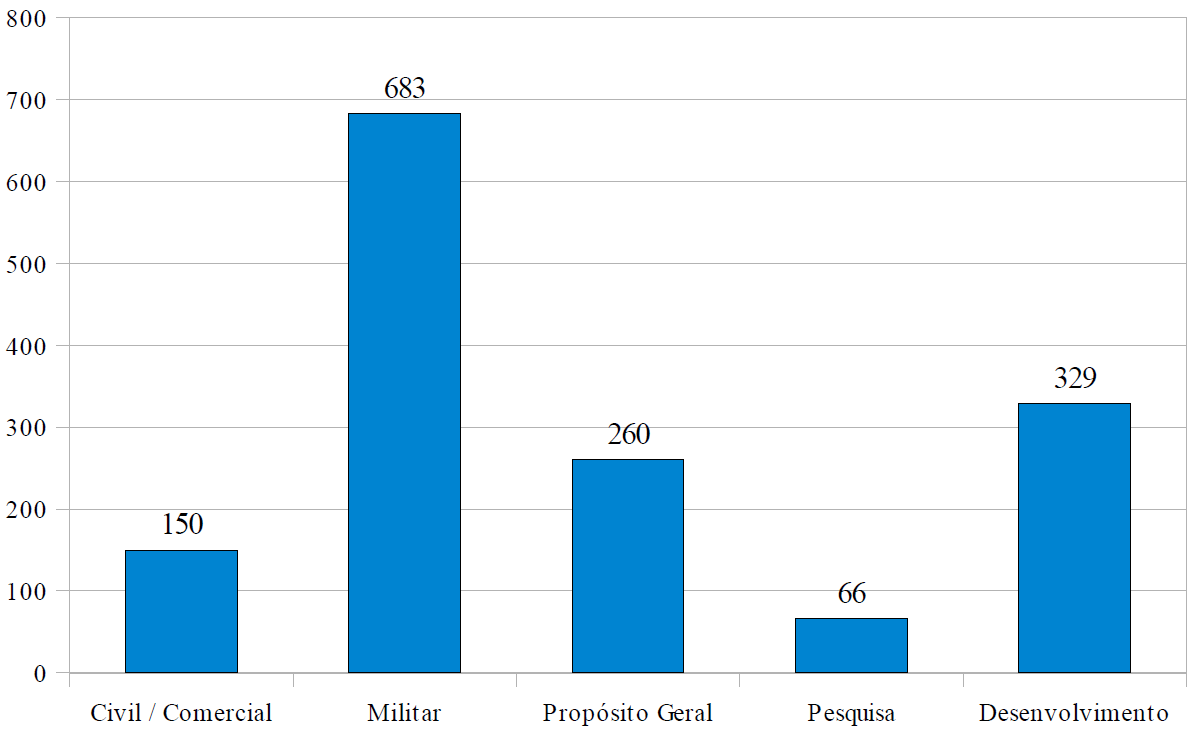
\includegraphics[width=13cm]{pictures/qt_uavs_app.png}
\caption{Quantidade de \vants por classe de aplicação. }
 \label{fig:qt_uav_app}
\end{figure}



\subsubsection{Desenvolvimento de \vants}

Diversas nações têm se destacado quanto ao desenvolvimento de VANTs. Os Estados Unidos é o país que atualmente possui mais aeronaves produzidas (386), e representa 32,44\% da
produção mundial de aeronaves não tripuladas. Outras nações como Israel (83 - 6,97\%),  França (77 unidades - 6,47\%), Rússia (59 unidades - 4,96\%) e Reino Unido (65 - 5,46\%) também têm apresentado resultados significativos quanto ao número de \vants produzidos. O Brasil, ainda iniciando suas pesquisa em \vants, possui 6 unidades produzidas, contabilizando apenas 0,5\% das aeronaves não tripuladas produzidas no mundo.

Na Tabela~\ref{tbl:country} encontram-se os dados resumidos do desenvolvimento de \vants em âmbito mundial \cite{Bryner2007}.

\begin{table}[h!]
\centering
	\begin{tabular}{| l | c | c |}
		\hline
		País & Número de Aeronaves & \% \\
		\hline
		EUA & 386 & 32,44 \\
		Israel & 83 & 6,97 \\
		França & 77 & 6,47 \\
		Reino Unido & 65 & 5,46 \\
		Iran & 38 & 3,19 \\
		Brasil & 6 & 0,50\\
		Outros Países & 535 & 44,97 \\
		\hline
	\end{tabular}

	\caption{Desenvolvimento de \vants por nação.}
	\label{tbl:country}
\end{table}